\chapter{Evaluation}
\label{chap:eval}

In this chapter, we evaluate the implementation of \textit{Ocelescope} through two user studies.
The studies examine how end-users work with the tool and how developers extend it by creating plugins.
In addition to the user studies, three plugins were developed as case studies that demonstrate the practical use of \textit{Ocelescope} for process mining tasks.

\section{User Evaluation}

Both user studies were conducted remotely using online forms. Each study followed the same structure and consisted of three parts.

\paragraph{Background Information}
At the beginning of each study, the form asked for basic information about the participant, such as their role, technical background, and experience with process mining or tool development.

\paragraph{Task}
After the background questions, the participants were directed to a small task list.
The tasks were hosted on the documentation page.
After completing the tasks, the participants returned to the main form.

\paragraph{Questionnaires}
After the task the participants answered several questions.
They rated how similar the task was to their previous work.
Usability and ease of use were measured using a TAM questionnaire~\cite{tam}, since TAM is a common instrument for assessing perceived usefulness and ease of use.
Finally, the participants were asked whether \textit{Ocelescope} would support their workflow and could give free-text feedback.

\subsection{Tool Evaluation}

This study evaluates \textit{Ocelescope} from the perspective of end-users who want to apply OCPM techniques without setting up individual research prototypes.
The goal is to test whether users can complete a basic workflow with the tool and to identify obstacles that hinder its use in practice.
The workflow was selected to cover key framework requirements from Table~4.4. In particular, the evaluation targets \textbf{setup and reliability} (BF-5a, BF-5b, BF-5c), \textbf{basic log handling} (BF-1a), and \textbf{plugin execution in \textit{Ocelescope}} (EX-1, EX-2a, EX-3c, EX-4a). Before starting the task, participants provided background information. The form collected their current role (e.g., student, researcher, or practitioner), their operating system, and their experience with other process mining tools. The questionnaire, task list, and full results are provided in the appendix (see \autoref{app:tool-evaluation}).

\subsubsection{Task Structure}
The task consisted of four steps. Participants were asked to:

\begin{enumerate}
	\item \textbf{Install} \textit{Ocelescope} by following the getting started instructions in the documentation.
	\item \textbf{Import} a plugin downloaded from the documentation page.
	\item \textbf{Load} one of the default OCELs.
	\item \textbf{Run} the plugin and export the result as a JSON file.
\end{enumerate}

\subsubsection{Results}

The survey included thirteen participants.
Most participants were researchers, followed by students and industry professionals.
Many also had previous experience with OCPM tools, which allowed them to compare \textit{Ocelescope} with other tools.
Figure~\ref{fig:tool-eval-pies} summarizes participant roles and their familiarity with OCPM tools.

\begin{figure}[h]
	\centering

	\begin{subfigure}[t]{0.48\textwidth}
		\centering
		\begin{tikzpicture}
			\pie[
				text=legend,
				radius=1.8,
				color={blue!40, green!40, orange!60}
			]{%
				23/Student,
				15/Practitioner,
				62/Researcher
			}
		\end{tikzpicture}
		\caption{Distribution of participant roles}
		\label{fig:role-distribution-pie}
	\end{subfigure}
	\hfill
	\begin{subfigure}[t]{0.48\textwidth}
		\centering
		\begin{tikzpicture}
			\pie[
				text=legend,
				radius=1.8,
				color={blue!40, orange!60}
			]{%
				77/Yes,
				23/No
			}
		\end{tikzpicture}
		\caption{Familiarity with OCPM tools}
		\label{fig:ocpm-familiarity-pie}
	\end{subfigure}

	\caption{Overview of participant background for the tool evaluation}
	\label{fig:tool-eval-pies}
\end{figure}

We first evaluate the questionnaire results reported in \autoref{tab:tam-table}. We assess ease of use in terms of installation and plugin execution, and usefulness in terms of the value of running plugins inside \textit{Ocelescope} for practitioners and researchers.

\begin{table}[h]
	\centering
	\small
	\renewcommand{\arraystretch}{1.25}
	\setlength{\tabcolsep}{4pt}

	\begin{tabularx}{\textwidth}{>{\raggedright\arraybackslash}X c r r}
		                               &                                  & \textbf{M}    & \textbf{SD}   \\ \hline

		\textbf{Perceived Usefulness}  &                                  & \textbf{3.76} & \textbf{0.68} \\ \hline
		\textbf{PU1:} Enables me to accomplish tasks more quickly
		                               & \likertbar[0.40]{3}{5}{5}{0}{0}  & 3.85          & 0.80          \\
		\textbf{PU2:} Improves my performance
		                               & \likertbar[0.40]{2}{4}{7}{0}{0}  & 3.62          & 0.77          \\
		\textbf{PU3:} Increases my productivity
		                               & \likertbar[0.40]{3}{4}{6}{0}{0}  & 3.77          & 0.83          \\
		\textbf{PU4:} Enhances my effectiveness
		                               & \likertbar[0.40]{2}{4}{7}{0}{0}  & 3.62          & 0.77          \\
		\textbf{PU5:} Makes it easier to apply process mining tools
		                               & \likertbar[0.40]{3}{8}{2}{0}{0}  & 4.08          & 0.64          \\
		\textbf{PU6:} It is useful for my work
		                               & \likertbar[0.40]{3}{3}{6}{1}{0}  & 3.62          & 0.96          \\ \hline

		\textbf{Perceived Ease of Use} &                                  & \textbf{4.17} & \textbf{0.75} \\ \hline
		\textbf{PEOU1:} Learning to operate it would be easy for me
		                               & \likertbar[0.40]{10}{1}{2}{0}{0} & 4.62          & 0.77          \\
		\textbf{PEOU2:} I find it easy to get it to do what I want
		                               & \likertbar[0.40]{6}{5}{1}{1}{0}  & 4.23          & 0.93          \\
		\textbf{PEOU3:} My interaction with it is clear and understandable
		                               & \likertbar[0.40]{4}{6}{1}{2}{0}  & 3.92          & 1.04          \\
		\textbf{PEOU4:} I find it flexible to interact with
		                               & \likertbar[0.40]{4}{4}{4}{1}{0}  & 3.85          & 0.99          \\
		\textbf{PEOU5:} It would be easy for me to become skillful at using it
		                               & \likertbar[0.40]{5}{4}{4}{0}{0}  & 4.08          & 0.86          \\
		\textbf{PEOU6:} I find it easy to use
		                               & \likertbar[0.40]{8}{2}{2}{1}{0}  & 4.31          & 1.03          \\
	\end{tabularx}

	\vspace{0.7em}
	\scriptsize
	\textcolor{orange}{\rule{7pt}{7pt}} Strongly disagree \quad
	\textcolor{yellow}{\rule{7pt}{7pt}} Disagree \quad
	\textcolor{lightgray}{\rule{7pt}{7pt}} Neutral \quad
	\textcolor{cyan}{\rule{7pt}{7pt}} Agree \quad
	\textcolor{blue}{\rule{7pt}{7pt}} Strongly agree

	\caption{
		TAM questionnaire results for the \textit{Ocelescope} evaluation. Values are reported as mean (M) and standard deviation (SD).
	}
	\label{tab:tam-table}
\end{table}


\paragraph{Questionnaire Summary}
The questionnaire results show generally positive ratings for \textbf{Perceived Ease of Use} (4.17, SD = 0.75).

Ratings for \textbf{Perceived Usefulness} were also positive (3.76, SD = 0.68). However, responses to the performance- and productivity-related items were more often neutral, indicating that participants were less certain about the added value of running plugins inside \textit{Ocelescope}.

Overall, \textbf{Perceived Ease of Use} was rated higher than \textbf{Perceived Usefulness}. In the following, we draw on the free-text feedback to explain these differences and to derive concrete improvement needs.

\paragraph{Installation Experience}
All participants were able to install \textit{Ocelescope} and complete the tasks without major issues.
Several participants mentioned that the setup was easy to follow, even without prior Docker experience.
This is consistent with the generally high \textbf{Perceived Ease of Use} ratings in \autoref{tab:tam-table}.
Only a few technical problems occurred, such as blocked ports.
These issues were solved by the participants, but they show that the documentation should include clearer troubleshooting guidance.
Participants also highlighted that not having to manage dependencies manually was a major benefit of the installation approach.

\paragraph{Lack of Interactive Feedback}
A recurring theme in the free-form feedback was missing feedback during interaction. Several participants expected the output to update when changing parameters, but results only changed after manually rerunning the plugin. This made it harder to understand the effect of parameter changes and slowed down exploration.
Some participants compared the workflow to ProM and found the separation of input and output familiar, but they missed ProM's interactive behaviour, where changes are reflected more immediately in the interface.
This helps explain the slightly lower ratings on the interaction-focused ease-of-use items (PEOU3, PEOU4).
It also helps explain the more neutral usefulness responses on performance and productivity, since limited feedback makes parameter exploration slower and less transparent.

\paragraph{Identified Usability Improvements}
The free-form feedback also included a few small suggestions for quick improvements. Most of them aim to reduce uncertainty during exploration by making the tool's current state more visible. The most relevant short-term improvements are:

\begin{itemize}
	\item a simple history of previous plugin runs and results,
	\item clearer feedback when cached results are displayed.
\end{itemize}

\paragraph{Summary of Observations}
Overall, users were able to install and use \textit{Ocelescope} successfully. The results show higher perceived ease of use than perceived usefulness. The free-form feedback suggests that this gap is mainly caused by missing interactive feedback during plugin execution. Improvements should therefore prioritize feedback and interactivity.

\subsection{Plugin Development Evaluation}

This study evaluates \textit{Ocelescope} from the perspective of plugin developers.
The goal is to examine whether participants can implement and integrate a plugin with the provided workflow and to identify obstacles that hinder plugin development in practice.
The task was selected to cover key framework requirements from Table~4.4.
In particular, the evaluation targets \textbf{plugin development and integration} (EX-3a, EX-3b, EX-3d), \textbf{interface generation and parameter handling} (EX-4a, EX-4b), and \textbf{packaging and execution} (EX-1, EX-2a).
Before starting the task, participants provided background information.
The form collected their current role, their programming experience, and their familiarity with Python and common tool chains.
It also asked which operating system they used and whether they had experience developing extensions or similar tools.
The questionnaire, task list, and full results are provided in the appendix (see \autoref{app:plugin-evaluation}).

\subsubsection{Task Structure}

The task consisted of implementing a small plugin that discovers a directly follows graph.
The task description used a short scenario in which participants had implemented a discovery algorithm for object-centric directly follows graphs and had a visualization written in Graphviz.
The goal was to embed this functionality into \textit{Ocelescope} as a plugin.

The task was split into the following steps:

\begin{enumerate}
	\item \textbf{Set up} the template plugin.
	\item \textbf{Specify} metadata.
	\item \textbf{Define} a resource with a visualization.
	\item \textbf{Implement} a plugin function.
	\item \textbf{Build and use} the plugin.
\end{enumerate}

To prevent participants from getting stuck the task list also contained small solution snippets.
After uploading the final plugin the form asked which of these solution steps were used.

\subsubsection{Results}

The survey was completed by eight participants.
Their roles were distributed across researchers, students, practitioners, and one non–process-mining user.
Most participants reported previous experience with process mining and described themselves as medium or highly skilled in Python.
Several also had experience with software development, although only two had previously built tools for OCPM.

\begin{figure}[h]
	\centering

	\begin{subfigure}[c]{0.48\textwidth}
		\centering
		\begin{tikzpicture}
			\pie[
				text=legend,
				radius=1.8,
				color={blue!40, green!40, orange!60, yellow!40}
			]{%
				25/Student,
				50/Researcher,
				12.5/Practitioner,
				12.5/Non PM User
			}
		\end{tikzpicture}
		\caption{Distribution of participant roles}
		\label{fig:role-distribution-pie-plugin}
	\end{subfigure}
	\hfill
	\begin{subfigure}[c]{0.48\textwidth}
		\centering
		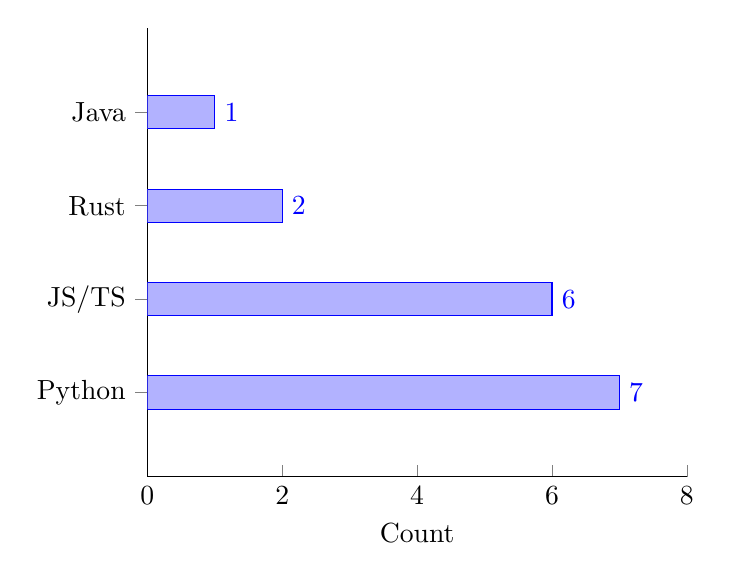
\begin{tikzpicture}
			\begin{axis}[
					xbar,
					xmin=0,
					xmax=8,
					xlabel={Count},
					symbolic y coords={Python,JS/TS,Rust,Java},
					ytick=data,
					bar width=12pt,
					nodes near coords,
					nodes near coords align={horizontal},
					enlarge y limits=0.3,
					axis x line*=bottom,
					axis y line*=left,
				]
				\addplot coordinates {
						(7,Python)
						(6,JS/TS)
						(2,Rust)
						(1,Java)
					};
			\end{axis}
		\end{tikzpicture}
		\caption{Main programming language of participants}
	\end{subfigure}

	\caption{Overview of participant background for the plugin development evaluation}
\end{figure}

Most participants mainly used Python and JavaScript or TypeScript in their daily work.
This indicates that the decision to support plugin development in Python was well aligned with the skills of typical users.

Participants also reported whether they used the solution hints provided in the task description. Three did not use any hints, two used all hints, one used only the final hint, and one used some of the intermediate hints. This variation suggests that the documentation and the task description were generally helpful, although some steps may require clearer explanations.

We first evaluate the questionnaire results reported in \autoref{fig:dev-tam-plugin-table}. We assess ease of use in terms of implementing and integrating a plugin, and usefulness in terms of how suitable \textit{Ocelescope} plugins are for implementing OCPM research prototypes. In the following, we draw on the free-form feedback to explain the main observations and derive concrete improvement needs.

\begin{table}[h]
	\centering
	\small
	\renewcommand{\arraystretch}{1.2}
	\setlength{\tabcolsep}{4pt}

	\begin{tabularx}{\textwidth}{>{\raggedright\arraybackslash}X c r r}
		                               &                                              & \textbf{$M$}  & \textbf{$SD$} \\ \hline

		\textbf{Perceived Usefulness}  &                                              & \textbf{5.56} & \textbf{0.82} \\ \hline
		\textbf{PU1:} Enables me to accomplish tasks more quickly
		                               & \likertscaleSeven[0.40]{0}{0}{0}{0}{3}{2}{3} & 6.00          & 0.93          \\
		\textbf{PU2:} Improve my performance
		                               & \likertscaleSeven[0.40]{0}{0}{1}{3}{1}{3}{0} & 4.75          & 1.16          \\
		\textbf{PU3:} Increases my productivity
		                               & \likertscaleSeven[0.40]{0}{0}{1}{2}{2}{2}{1} & 5.00          & 1.31          \\
		\textbf{PU4:} Enhance my effectiveness
		                               & \likertscaleSeven[0.40]{0}{0}{1}{1}{0}{4}{2} & 5.62          & 1.41          \\
		\textbf{PU5:} Make it easier to develop OCPM tools
		                               & \likertscaleSeven[0.40]{0}{0}{0}{0}{1}{3}{4} & 6.38          & 0.74          \\
		\textbf{PU6:} It is useful for my work
		                               & \likertscaleSeven[0.40]{0}{0}{0}{2}{0}{5}{1} & 5.62          & 1.06          \\ \hline

		\textbf{Perceived Ease of Use} &                                              & \textbf{5.60} & \textbf{0.67} \\ \hline
		\textbf{PEOU1:} Learning to write a plugin would be easy for me
		                               & \likertscaleSeven[0.40]{0}{0}{0}{0}{4}{2}{2} & 5.75          & 0.89          \\
		\textbf{PEOU2:} Easy to get a plugin to do what I want
		                               & \likertscaleSeven[0.40]{0}{0}{0}{2}{4}{1}{1} & 5.12          & 0.99          \\
		\textbf{PEOU3:} Development process is clear and understandable
		                               & \likertscaleSeven[0.40]{0}{0}{0}{1}{2}{2}{3} & 5.88          & 1.13          \\
		\textbf{PEOU4:} The plugin system is flexible to work with
		                               & \likertscaleSeven[0.40]{0}{0}{0}{1}{2}{5}{0} & 5.50          & 0.76          \\
		\textbf{PEOU5:} Easy to become skillful at writing plugins
		                               & \likertscaleSeven[0.40]{0}{0}{0}{1}{4}{2}{1} & 5.38          & 0.92          \\
		\textbf{PEOU6:} Overall, plugin development is easy
		                               & \likertscaleSeven[0.40]{0}{0}{0}{0}{3}{2}{3} & 6.00          & 0.93          \\
	\end{tabularx}

	\vspace{0.7em}
	\scriptsize
	\textcolor{red}{\rule{7pt}{7pt}} Extremely disagree \quad
	\textcolor{orange}{\rule{7pt}{7pt}} Quite disagree \quad
	\textcolor{yellow}{\rule{7pt}{7pt}} Slightly disagree \quad
	\textcolor{lightgray}{\rule{7pt}{7pt}} Neither agree nor disagree \quad
	\textcolor{cyan!60}{\rule{7pt}{7pt}} Slightly agree \quad
	\textcolor{cyan}{\rule{7pt}{7pt}} Quite agree \quad
	\textcolor{blue}{\rule{7pt}{7pt}} Extremely agree

	\caption{TAM questionnaire results for \textit{Ocelescope} plugin development ($n=8$). $M$ denotes the sample mean and $SD$ the sample standard deviation.}
	\label{fig:dev-tam-plugin-table}
\end{table}

\paragraph{Questionnaire Summary}
The questionnaire results show generally positive ratings for \textbf{Perceived Ease of Use} ($M = 5.60$, $SD = 0.67$). Items related to learning and overall ease received the highest ratings (PEOU1, PEOU3, PEOU6). In contrast, getting a plugin to do what participants wanted was rated lower (PEOU2), which suggests some remaining friction during implementation.

\textbf{Perceived Usefulness} was rated similarly positive ($M = 5.56$, $SD = 0.82$). Participants rated the support for developing OCPM tools particularly high (PU5, PU1). Ratings were lower for performance- and productivity-related items (PU2, PU3), which suggests that participants still faced challenges when developing plugins in an effective and productive way.

Overall, Perceived Ease of Use was rated slightly higher than Perceived Usefulness, but both constructs are close.
In the following, we draw on the free-form feedback to explain why learning and basic integration were rated highly, while implementation details and efficient development still caused difficulties. We then derive improvement needs to make \textit{Ocelescope} more useful for developing OCPM tools in a productive way.

\paragraph{Main Issues Identified}
The free-text feedback helps explain why learning and basic integration were rated highly (PEOU1, PEOU3, PEOU6), while ratings related to getting the plugin to behave as intended and working efficiently were lower (PEOU2, PU2, PU3).

First, several participants described the iteration cycle as slow.
Small changes often required rebuilding the plugin package and importing it again, which made experimentation less fluid and affected how productive the workflow felt.
A common suggestion was a development mode with automatic reload or a simpler way to update code during development.

Second, participants reported uncertainty around input configuration.
Some steps were described as unclear, especially when participants had limited tool development experience or when their editor did not provide helpful guidance.
This aligns with the lower rating for getting a plugin to do what participants wanted (PEOU2).

Third, participants missed feedback while running or testing their plugin.
Long-running tasks did not show visible progress, and some participants were unsure whether the system was still working or had become unresponsive.

Finally, some participants questioned how well the plugin workflow scales to more complex tools and visualizations.

\paragraph{Minor Improvements}
Participants also suggested smaller improvements that would reduce uncertainty during development and usage.

One participant asked for clearer behavior when reuploading a plugin, especially when the same version is uploaded again. Suggested improvements included an explicit overwrite prompt and clearer naming of the build artifact.

Some comments also pointed to documentation and interface clarity. Participants were not always sure how to use exported resources, and a few interface elements were described as unclear in their purpose.


\paragraph{Summary of Observations}

Overall, participants were able to complete the plugin development task successfully.
Many comments emphasized that \textit{Ocelescope} reduces boilerplate work, especially when setting up a usable interface around existing code.
The step-by-step guide and the template structure were also described as helpful.
When asked whether the plugin framework could support tools they are currently developing or plan to develop in the future, all participants responded positively.
At the same time, a few comments indicate that this support may depend on the complexity of the planned tool, especially when more advanced visualizations or interaction are required.

The feedback also points to improvements that would make plugin development feel more effective and productive, which aligns with the lower ratings on PU2 and PU3.
The most important areas are faster iteration during development, clearer guidance for input configuration, and better feedback while tasks run.
Addressing these points would reduce friction in the development workflow and strengthen the plugin framework as a basis for research tools.

\section{Proof of Concepts}

In addition to the evaluation, two plugins were developed as proof of concepts.
These plugins demonstrate that \textit{Ocelescope} not only supports standard use cases, but can also be used to implement more specialised functionality.
The goal of these prototypes was to test how well the framework supports extensions of OCEL and the integration of Rust implementations through Python bindings.

\subsection*{Qnet Plugin}

The Qnet plugin serves as a proof of concept for extending OCELs in \textit{Ocelescope}, as required by requirement \req{BF-1b} (\autoref{tab:requirements}).
It implements an OCEL that is extended with object quantities and quantity operations, following the ideas described in~\cite{qrpm}.

The quantity extension was implemented as an OCEL extension for OCELs in the XML format. During import, the plugin checks whether the extension data is present and parses it into pandas dataframes.
These tables are exposed as attributes of the extension class.
The plugin provides one function that discovers a Qnet based on an OCEL containing the extension and a selected item type.
The item type is offered as a computed field that lists all available types in the log.
The plugin returns the discovered Qnet together with a dot visualization.

The development of the Qnet plugin showed that the current OCEL extension system is useful for extending OCELs. It provides a clear structure for defining extensions and offers the benefit of automatic generator functionality for extended logs. Once the extension is defined, new logs can be created manually with support from the \textit{Ocelescope} Python package. The plugin also highlights the usefulness of computed fields, because they allow the creation of dynamic input fields for extensions.

During the development, the following improvement opportunities were identified:

\begin{itemize}
	\item The implementation of an extension could be made simpler. At the moment, the import, export, and validation functions must be implemented manually for each of the three OCEL extension formats. This is time-consuming and error-prone. A schema language could be used to describe extension data. From such a schema, the required functions could be generated automatically. This would allow extensions to be reused across plugins in a similar way as resources.
	\item Extensions would benefit from a specialised computed field type. This would make the creation of extension-aware input fields easier.
	\item The user interface in the \textit{Ocelescope} web view needs minor improvements. Extensions are only loaded after the registration of the extension. This caused confusion because logs that were loaded before did not show the extension fields, and some input fields in plugin forms stayed empty. A clearer indication of which fields depend on an extension would help users understand the behaviour.
\end{itemize}

\subsection*{OC-DECLARE}

As a second proof of concept, the OC-DECLARE plugin demonstrates the integration of a Rust implementation through Python bindings in \textit{Ocelescope}, as required by requirement \req{EX-6} (\autoref{tab:requirements}).
It demonstrates that \textit{Ocelescope} can be used to build plugins that rely on external implementations in other programming languages. OC-DECLARE extends the DECLARE approach to the object-centric setting and was introduced in~\cite{ocdeclare}. The implementation used in this plugin was written in Rust and exposed to Python through the \texttt{oc-declare} Python library.\footnote{\url{https://pypi.org/project/oc-declare}}

The plugin integrates the Python wheel to make the full OC-DECLARE functionality available. It defines a resource called \textit{DeclareConstraints}, which stores a set of OC-DECLARE constraint definitions. The resource is visualised as a table in the user interface.

Based on this resource, the plugin implements the following functions:

\begin{itemize}
	\item \textbf{Discover Constraints:} automatically discovers OC-DECLARE constraints from an event log and returns them as a \textit{DeclareConstraints} resource.
	\item \textbf{Create Constraints:} allows users to manually define constraints through an OCEL-based input form.
	\item \textbf{Check Constraints:} receives an OCEL and a set of constraints and checks whether they conform to one another.
\end{itemize}

When executed, these functions call the corresponding Python functions of the OC-DECLARE package.
Since these functions expect file paths, the OCEL instance must first be written to a temporary file.
The OC-DECLARE module then parses the file again into its own OCEL representation.
While this is not ideal, it still provides a working integration and shows that external Rust libraries can be used through Python bindings in \textit{Ocelescope}.
